\documentclass{beamer}
\usepackage{../common_slides}


\title{Text Classification\\ + \\ Machine Learning Review }
\date{}
\author{CS 287}
\begin{document}


\begin{frame}
  \titlepage
\end{frame}

\section{Text Classification }

\begin{frame}
\begin{quote}
   Earn a Degree based on your Life Experience

  Obtain a Bachelor's, Master's, MBA, or PhD based on your present
    knowledge and life experience.

    No required tests, classes, or books. Confidentiality assured.

    Join our fully recognized Degree Program.

    Are you a truly qualified professional in your field but lack the
    appropriate, recognized documentation to achieve your goals?

    Or are you venturing into a new field and need a boost to get your
    foot in the door so you can prove your capabilities?

    Call us for information that can change your life and help you to
    achieve your goals!!!

    CALL NOW TO RECEIVE YOUR DIPLOMA WITHIN 30 DAYS
\end{quote}
\end{frame}


\begin{frame}{Sentiment}
  \structure{Good Sentences}
  \begin{itemize}
  \item   A thoughtful, provocative, insistently humanizing film. 
  \item   Occasionally melodramatic, it's also extremely effective.
    \item   Guaranteed to move anyone who ever shook, rattled, or rolled.   
  \end{itemize}

  \alert{Bad Sentences}
  \begin{itemize}
  \item A sentimental mess that never rings true.  
  \item This 100-minute movie only has about 25 minutes of decent material.
  \item Here, common sense flies out the window, along with the hail of
    bullets, none of which ever seem to hit Sascha.
  \end{itemize}
\end{frame}

\begin{frame}{Multiclass Sentiment}
    \begin{itemize}
    \item 
      $\star \star \star \star$

      I visited The Abbey on several occasions on a visit to Cambridge and found it to be a solid, reliable and friendly place for a meal.
      
    \item $\star \star$ 

      However, the food leaves something to be desired. A very obvious menu and average execution

    \item $\star \star \star \star \star$

      Fun, friendly neighborhood bar. Good drinks, good food, not too pricey. Great atmosphere!
  \end{itemize}
\end{frame}

% \begin{frame}{Practical: Document Categorization}
% \end{frame}




\begin{frame}{Text Categorization}
  \begin{itemize}
  \item Straightforward setup. 
  \item Lots of practical applications:
    \begin{itemize}
    \item Spam Filtering
    \item Sentiment
    \item Text Categorization
    \item e-discovery
    \item Twitter Mining 
    \item Author Identification
    \item $\ldots$
    \end{itemize}
  \item Introduces machine learning notation.
  \end{itemize}

  \vspace{0.24cm}

  However, a relatively solved problem these days.
\end{frame}


\section{Preliminaries: Machine Learning for NLP}

\subsection{Features and Preprocessing}

\begin{frame}{Preliminary Notation}
  \begin{itemize}
  \item $\boldb, \boldm$;  bold letters for vectors.
  \item $\boldB, \boldM$;  bold capital letters for matrices.
  \item $\mcB, \mcM$;  script-case for sets.
  \item $B, M$; capital letters for random variables.
  \item $b_i, x_i$; lower case for scalars or indexing into vectors.
  \end{itemize}


  \begin{itemize}
  \item $\bolddelta(i)$; one-hot vector at position i
    \[\bolddelta(2) = \left[ 0; 1; 0; \dots \right]\] 
  \item $\indicator(x = y)$; indicator 1 if $x = y$, o.w. 0

  \end{itemize}


\end{frame}


\begin{frame}{Text Classification}

  \begin{enumerate}
  \item Extract pertinent information from the sentence. 
    \air 

  \item Use this to construct an input representation.
    \air

  \item Classify this vector into an output class.
  \end{enumerate}

  \pause
  \air


  \textbf{Input Representation:}
  \begin{itemize}
  \item Conversion from  text into a mathematical representation?
  \item Main focus of this class, representation of language
  \item Point in coming lectures: \textit{sparse} vs. \textit{dense} representations
  \end{itemize}

  % Throughout this class, 
  % \begin{itemize}
  % \item $\mcX = \reals^{\din}$
  % \item $\mcY \subset \{0, 1\}^{\dout}$
  % \end{itemize}
\end{frame}





\begin{frame}{Sparse Features (Notation from YG)}
  \begin{itemize}
   
  \item   $\mcF$; a discrete set of features values. 
  \item   $f_1\in\mcF, \ldots , f_k\in\mcF$; active features for input. 
    
    \air 
    
    For a given sentence, let $f_1, \ldots f_k$  be the relevant features.  Typically $k << |\mcF|$.

\air

  \item Sparse representation of the input defined as,
    \[\boldx = \sum_{i=1}^k \bolddelta(f_i) \]
  \item $\boldx \in \reals^{1\times \din}$; input representation 
  \end{itemize}

  % In this section we consider \textbf{sparse} features. Informally this means
  % $\din$ is large, and $\boldx$ is sparse.   
\end{frame}



\begin{frame}{Features 1: Sparse Bag-of-Words Features}
  Representation is counts of input words, 
  \begin{itemize}
  \item $\mcF$; the vocabulary of the language.
  \item $\boldx = \sum_{i} \bolddelta(f_i)$ 
  \end{itemize}

  Example: Movie review input, 
  \begin{center}
    \texttt{A sentimental mess}
    \[ \boldx = \bolddelta(\texttt{word:A}) + \bolddelta(\texttt{word:sentimental}) +
    \bolddelta(\texttt{word:mess}) \] 
    \[ \boldx^\top =\begin{bmatrix} 1 \\ \vdots
        \\ 0\\ 0 \\ \end{bmatrix} +\begin{bmatrix} 0 \\
        \vdots \\ 0\\ 1 \\ \end{bmatrix} +
     \begin{bmatrix} 0 \\ \vdots \\ 1\\ 0 \\ \end{bmatrix} 
    =\begin{bmatrix} 1 \\ \vdots \\ 1 \\ 1 \\ \end{bmatrix} 
    \begin{matrix*}[l] \mathrm{\texttt{word:A}} \\ \vdots \\ \mathrm{\texttt{word:mess}} \\ \mathrm{\texttt{word:sentimental}} \\ \end{matrix*}
     \]
  \end{center}
\end{frame}


\begin{frame}{Features 2: Sparse Word Properties}
  Representation can use specific aspects of text.
  \begin{itemize}
  \item $\mcF$; Spelling, all-capitals, trigger words, etc. 
  \item $\boldx = \sum_{i} \bolddelta(f_i)$ 
  \end{itemize}

  Example: Spam Email

  \begin{center}
    \texttt{Your diploma puts a UUNIVERSITY JOB PLACEMENT COUNSELOR at
      your disposal.}
  \end{center}
  \[  \boldx = \bolddelta(\texttt{misspelling}) + \bolddelta(\texttt{allcapital}) + \bolddelta(\texttt{trigger:diploma}) + \ldots\]
  \[
  \boldx^\top = 
 \begin{bmatrix} 0 \\ \vdots \\ 1\\  0 \\  \end{bmatrix} + 
 \begin{bmatrix} 0 \\ \vdots \\ 0\\ 1 \\  \end{bmatrix} +
 \begin{bmatrix} 1 \\ \vdots \\ 0\\  0 \\  \end{bmatrix} = 
 \begin{bmatrix} 1 \\ \vdots \\ 1 \\ 1 \\  \end{bmatrix}     \begin{matrix*}[l] \mathrm{\texttt{misspelling}} \\ \vdots \\ \mathrm{\texttt{capital}} \\ \mathrm{\texttt{word:diploma}} \\ \end{matrix*}
  \]
\end{frame}

\subsection{Output}

\begin{frame}{Text Classification: Output Representation}
  \begin{enumerate}
  \item Extract pertinent information from the sentence. 
    \air 

  \item Use this to construct an input representation.
    \air

  \item Classify this vector into an output class.
  \end{enumerate}

  \air


  \textbf{Output Representation:}

  \begin{itemize}
  \item How do encode the output classes?
  \item We will use a one-hot output encoding.
  \item In future lectures, efficiency of output encoding.
  \end{itemize}
\end{frame}




\begin{frame}{Output Class Notation}
  \begin{itemize}
  \item $\mcC = \{1, \ldots, \dout\}$; possible output classes
  \item $c \in \mcC$; always one true output class 
  \item $\boldy = \bolddelta(c) \in \reals^{1\times \dout}$; true one-hot output representation

  % \item Note: when classes are words, we call them \textit{word types}. 
  \end{itemize}
\end{frame}

\begin{frame}{Output Form: Binary Classification}

  Examples: spam/not-spam, good review/bad review, relevant/irrelevant document, many others.   
  \begin{itemize}
  \item $\dout = 2$; two possible classes
  \item In our notation,
    \begin{eqnarray*} 
    bad \ \ c = 1 & \  \boldy &= \begin{bmatrix} 1 & 0  \end{bmatrix}  \mathrm {\ vs. \ } \\
    good \ c = 2 & \boldy &= \begin{bmatrix} 0  & 1  \end{bmatrix} 
   \end{eqnarray*} 
   \item Can also use a single output \textit{sign} representation with $\dout = 1$ 
  \end{itemize}

\end{frame}


% \begin{frame}{Step 1: Feature Extraction}
%   \begin{itemize}
%   \item Let $\mcV$ be the vocabulary of our language.  
%   \item  Let $w_1, \ldots, w_m$ be a sentence, where 
%     $w_i \in \{1,\ldots, |\mcV|\}$.
%   \item 
%   \end{itemize}
% \end{frame}



% \begin{frame}{Step 2: Learn a Classifier}
%   Next we map a representation $\boldx$ to a output $\boldy$.
  
%   The output $\boldy \in \reals^\dout$ where $\dout$ is the number of 
%   \textit{classes}. 

%   Generally $\boldy$ will be a one-hot vector. 

%   \begin{itemize}
%   \item $\dout = 2$; two possible classes
%     \[\begin{bmatrix} 1 \\ 0  \end{bmatrix}  \mathrm {\ vs. \ } 
%    \begin{bmatrix} 0 \\ 1  \end{bmatrix} \]
%   \end{itemize}

%   For instance spam/not-spam, good review/bad review, relevant/irrelevant

% \end{frame}

\begin{frame}{Output Form: Multiclass Classification}
  Examples: Yelp stars, etc.
  \begin{itemize}
  \item $\dout = 5$; for examples
  \item In our notation, one star, two star...
    \begin{eqnarray*} 
      \star \ c = 1 & \  \boldy &= \begin{bmatrix} 1 & 0 & 0 & 0 & 0  \end{bmatrix}  \mathrm {\ vs. \ } \\
    \star \star \ c = 2 & \boldy &=    \begin{bmatrix} 0 & 1 & 0 & 0 & 0 \end{bmatrix} \ldots
   \end{eqnarray*} 
  \end{itemize}
  Examples: Word Prediction (Unit 3)
  \begin{itemize}
  \item $\dout > 100,000$; 
  \item In our notation, $\mcC$ is vocabulary and each $c$ is a word.   
    \begin{eqnarray*} 
      the \ c = 1 & \  \boldy &= \begin{bmatrix} 1 & 0 & 0 & 0 & \ldots & 0  \end{bmatrix}  \mathrm {\ vs. \ } \\
      dog \ c = 2 & \boldy &=    \begin{bmatrix} 0 & 1 & 0 & 0 & \ldots & 0 \end{bmatrix} \ldots
   \end{eqnarray*} 
  \end{itemize}
\end{frame}

\begin{frame}{Evaluation}
  \begin{itemize}
  \item Consider evaluating accuracy on outputs $\boldy_1, \ldots, \boldy_n$. 

  \item Given a predictions $\hat{c_1} \ldots \hat{c_n}$ we measure 
  accuracy as,
  
  \[ \sum_{i=1}^n \frac{\indicator(\bolddelta(\hat{c}_i) = \boldy_i)}{ n} \] 

  \item Simplest of  several different metrics we will explore in the class. 
  \end{itemize}
\end{frame}


% \begin{frame}{Example: Multiclass Classification}
%   More interestingly we will also consider multiclass where $\dout > 2$

%   \begin{itemize}
%   \item $\dout = 5$; yelp review.
%     \[\begin{bmatrix} 1 \\ 0 \\0 \\0 \\0  \end{bmatrix}  \mathrm {\ vs. \ } 
%    \begin{bmatrix} 0 \\ 1 \\0 \\0 \\0  \end{bmatrix}  \mathrm {\ vs. \ } \ldots \] 
%   \end{itemize}
%   For instance five star review, etc. 
% \end{frame}




\section{Classification}


\begin{frame}{Supervised Machine Learning}
  Let, 
  \begin{itemize}
  \item $(\boldx_1, \boldy_1), \ldots, (\boldx_n, \boldy_n)$; training data
  \item $\boldx_i \in \reals^{1 \times \din}$;  input representations  
  \item $\boldy_i \in \reals^{1 \times \dout}$; true output representations (one-hot vectors)
  \end{itemize}

  Goal: Learn a classifier from input to output classes.  

  \air
  \air

  Note:
  \begin{itemize}
  \item $\boldx_i$ is an input vector $x_{i, j}$ is element of the vector, or just $x_j$ when there is a clear single input .
  \item Practically, store design matrix $\boldX \in \reals^{n    \times \din}$ and output classes.
  \end{itemize}


\end{frame}


\begin{frame}{Experimental Setup}
  
  \begin{itemize}
  \item Data is split into three parts training, validation, and test.
  \item Experiments are all run on training and validation, test is final output.

  \item For assignments, full training and validation data, and only inputs for test.
  \end{itemize}
  
  For very small text classification data sets,
  \begin{itemize}
  \item Use K-fold cross-validation. 
    \begin{enumerate}
    \item Split into K folds (equal splits).
    \item For each fold, train on other K-1 folds, test on current fold. 
    \end{enumerate}
  \end{itemize}
\end{frame}

\subsection{Linear Models}

\begin{frame}{Linear Models for Classification}
  Linear model,
  \[\hat{\boldy} = f(\boldx \boldW + \boldb)\]    
  \begin{itemize}
  \item $\boldW \in \reals^{\din \times \dout}, \boldb \in \reals^{1 \times \dout}$; model parameters
  \item $f: \reals^{\dout} \mapsto \reals^{\dout}$; activation function 
  \item Sometimes $\boldz = \boldx \boldW + \boldb$ informally ``score'' vector. 
  \item Note $\boldz$ and $\hat{\boldy}$ are not one-hot.
  \end{itemize}

  \air 

  Class prediction,
  \[ \hat{c} = \argmax_{i \in \mcC} \hat{y_i}  = \argmax_{i \in \mcC} (\boldx \boldW + \boldb)_i    \]
\end{frame}


\begin{frame}{Interpreting Linear Models}
  Parameters give scores to possible outputs,
  \begin{itemize}
  \item $W_{f, i}$ is the score for sparse feature $f$ under class $i$
  \item $b_i$ is a prior score for class $i$  
  \item $\hat{y}_i$ is the total score for class $i$
  \item $\hat{c}$ is highest scoring class under the linear model.
  \end{itemize}

  Example:
  \begin{itemize}
  \item For single feature score, \[[\beta_1, \beta_2 ] = \bolddelta(\texttt{word:dreadful}) \boldW,\]
    Expect $\beta_1 > \beta_2$ (assuming $2$ is class \textit{good}). 
    
  \end{itemize}
\end{frame}



\begin{frame}{Probabilistic Linear Models} 
  % Estimate
  Can estimate a linear model probabilistically,

  \begin{itemize}
  \item Let output be a random variable $Y$, with sample space $\mcC$. 
  \item Representation be a random vector $X$. 
  \item (Simplified frequentist representation)
  \item Interested in estimating parameters $\theta$,
      \[ P(Y | X; \theta) \] 
  \end{itemize}
  Informally we use $p(\boldy=\bolddelta(c) | \boldx)$ for 
  $P(Y = c | X = \boldx)$.
  
\end{frame}



\begin{frame}{Generative Model. Joint Log-Likelihood as Loss } 
  % Estimate 
  \begin{itemize}
  \item $(\boldx_1, \boldy_1), \ldots, (\boldx_n, \boldy_n)$; supervised data
  \item Select parameters to maximize likelihood of training data.
    \[ \mathcal{L}(\theta) =  - \sum_{i=1}^n \log p(\boldx_i, \boldy_i; \theta) \] 
  For linear models $\theta = (\boldW, \boldb)$ 

  \item Do this by minimizing negative log-likelihood (NLL).
    \[ \argmin_\theta \mathcal{L}(\theta)\] 
  \end{itemize}
\end{frame}


\subsection{Linear Model 1: Naive Bayes}

\begin{frame}{Multinomial Naive Bayes } 
  % Estimate 
  Reminder, joint probability chain rule,  

  \[ p(\boldx, \boldy) = p(\boldx | \boldy) p(\boldy) \] 


    \pause
  For a sparse features, with observed classes we can write as,
  
  \begin{eqnarray*}
    p(\boldx, \boldy) &=& p(x_{f_1}=1, \ldots, x_{f_k}=1 | \boldy=\bolddelta(c) ) p(\boldy=\bolddelta(c)) =\\
     &=& \prod_{i=1}^k p(x_{f_i}=1 | x_{f_1}=1, \ldots, x_{f_{i-1}}=1, \boldy=\bolddelta(c)) p(\boldy=\bolddelta(c)) \approx \\
     &=& \prod_{i=1}^k p(x_{f_i} =1| \boldy) p(\boldy)  
  \end{eqnarray*}

  
  First is by chain-rule, second is by independence assumption.


\end{frame}




\begin{frame}{Estimating Multinomial Distributions} 
  Let $S$ be a random variable with sample space $\mcS$ and 
  we have observations $s_1, \ldots, s_n$, 


  \begin{itemize}
  \item $P(S=s; \theta) = \mathrm{Cat} (s;\theta)$; parameterized as a multinomial distribution.
    \pause
  \item Minimizing NLL for multinomial (MLE) for data has a closed-form.

    \[ P(S=s; \theta) = \mathrm{Cat} (s;\theta) = \sum_{i=1}^n \frac{\indicator(s_i = s)}{n} \]

  \item Exercise: Derive this by minimizing $\mathcal{L}$. 

  \end{itemize}

  \begin{itemize}
  \item Also called categorical or multinoulli (in Murphy).
  \end{itemize}
\end{frame}



\begin{frame}{Multinomial Naive Bayes}
  \begin{itemize}
  \item  Both  $p(\boldy)$ and $p(\boldx | \boldy)$ are
    parameterized as multinomials.
    
  \item Fit first as,
    \[p(\boldy = \bolddelta(c)) = \sum_{i = 1}^n \frac{1(\boldy_i = c)}{n}\]
    \pause

  \item Fit second using count matrix $\boldF$ ,
    \begin{itemize}
      \item Let \[F_{f,c} = \sum_{i = 1}^n \indicator(\boldy_i = c) \indicator(x_{i, f} = 1) \mathrm{\ for all\ } c\in \mcC, f\in \mcF\] 
      \item Then,
      \[p(x_f = 1 | \boldy=\bolddelta(c)) = \frac{F_{f, c}}{\displaystyle \sum_{f' \in \mcF} F_{f',c}}  \]     
    \end{itemize}
  \end{itemize}
\end{frame}


\begin{frame}{Alternative:  Multivariate Bernoulli Naive Bayes}
  \begin{itemize}
  \item  Both  $p(\boldy)$ is multinomial as above 
    and $p(x_f | \boldy)$ is Bernoulli over each features .
   
  \item Fit class as Categorical,
    \[p(\boldy = \bolddelta(c)) = \sum_{i = 1}^n \frac{1(\boldy_i = c)}{n}\]
    \pause
    
  \item Fit features using count matrix $\boldF$ ,
    \begin{itemize}
      \item Let \[F_{f,c} = \sum_{i = 1}^n \indicator(\boldy_i = c) \indicator(x_{i, f} = 1) \mathrm{\ for all\ } c\in \mcC, f\in \mcF\] 
      \item Then,
      \[p(x_f | \boldy=\bolddelta(c)) = \frac{F_{f, c}}{\displaystyle \sum_{i = 1}^n \indicator(\boldy_i = c)}  \]     
    \end{itemize}
  \end{itemize}
\end{frame}


\begin{frame}{Getting a Conditional Distribution}
  \begin{itemize}
  \item Generative models estimates of $P(X, Y)$, we want $P(Y | X)$. 
  \item
  Bayes Rule,

  \[  p(\boldy | \boldx) = \frac{ p(\boldx | \boldy)  p(\boldy)}{ p(\boldx)}  \] 
  
\item  In log-space,

  \[ \log p(\boldy | \boldx) = \log p(\boldx| \boldy) + \log p(\boldy) - \log p(\boldx)  \] 
  \end{itemize}
  
\end{frame}

\begin{frame}{Prediction with Naive Bayes}
  \begin{itemize}
  \item  For prediction, last term is constant, so 
  
  \[ \argmax_c \log p(\boldy =\bolddelta(c) | \boldx) = \log p(\boldx | \boldy=\bolddelta(c)) + \log p(\boldy=\bolddelta(c))  \] 

   \item  Can write as linear model,
     \[ W_{f, c} =  \log p(x_f = 1 | \boldy=c)  \mathrm{\ for\ all\  }c\in \mcC, f\in\mcF \] 
     \[ b_c = \log p(\boldy=\bolddelta(c))  \mathrm{\ for\ all\  }c\in \mcC \] 
   \end{itemize}
\end{frame}


\begin{frame}{Getting a Conditional Distribution}
  \begin{itemize}
  \item 

  What if we want conditional probabilities? 
  \[  p(\boldy | \boldx) = \frac{ p(\boldx | \boldy)  p(\boldy)}{ p(\boldx)} = \frac{ p(\boldx | \boldy)  p(\boldy)}{ \sum_{c' \in \mcC} p(\boldx, \boldy=\delta(c'))} \] 

  \item Denominator is acquired by renormalizing,
  \[  p(\boldy | \boldx) \propto p(\boldx | \boldy)  p(\boldy)  \] 

  \end{itemize}
\end{frame}

\begin{frame}{Practical Aspects: Calculating Log-Sum-Exp}


  \begin{itemize}

  \item  Because of numerical issues, calculate in log-space,
  \[  f(\boldz) =  \log p(\boldy=\delta(c) | \boldx) = \log z_c  - \log \sum_{c' \in \mcC} \exp(z_{c'})  \] 
  where for naive Bayes
  \[ \boldz = \boldx \boldW + \boldb\] 
  \end{itemize}
  \pause
  
  \begin{itemize}
  \item However hard to calculate, \[\log \sum_{c' \in \mcC} \exp(\hat{z}_{c'})\]
  \item Instead 
    \[\log \sum_{c' \in \mcC} \exp(\hat{y}_{c'} - M) + M\] where $M = \max_{c'\in\mcC} \hat{z}_{c'}$ 
  \end{itemize}
\end{frame}


\begin{frame}{Digression: Zipf's Law}
  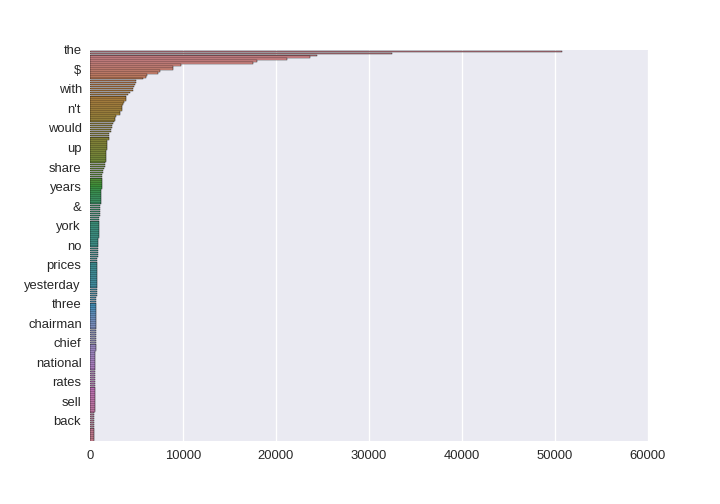
\includegraphics[width=\textwidth]{../notebooks/zipf}
\end{frame}

\begin{frame}{Laplace Smoothing}
  Method for handling the long tail of words by distributing mass, 
  \begin{itemize}
  \item  Add a value of $\alpha$ to each element in the sample space before normalization.

    \[ \theta_s =  \frac{\alpha + \sum_{i=1}^n \indicator(s_i = s)}{\alpha|\mcS|  + n} \]
    
  \item (Similar to Dirichlet prior in a Bayesian interpretation.) 
  \end{itemize}
  
\pause
  For naive Bayes:
  \[\hat{\boldF} = \alpha + F\]
 
\end{frame}

\begin{frame}{Naive Bayes In Practice}
  \begin{itemize}
  \item Very fast to train
  \item Relatively interpretable.
  \item Performs quite well on small datasets

  \begin{figure}
    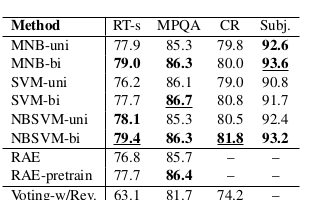
\includegraphics{data}
    \caption{  (RT-S [movie review], CR [customer reports], MPQA [opinion polarity], SUBJ [subjectivity])}
  \end{figure}
\end{itemize}

\end{frame}

\end{document}

